%%%%%%%%%%%%%%%%%%%%%%%%%%%%%%%%%%%%%%%%%
% Short Sectioned Assignment LaTeX Template Version 1.0 (5/5/12)
% This template has been downloaded from: http://www.LaTeXTemplates.com
% Original author:  Frits Wenneker (http://www.howtotex.com)
% License: CC BY-NC-SA 3.0 (http://creativecommons.org/licenses/by-nc-sa/3.0/)
%%%%%%%%%%%%%%%%%%%%%%%%%%%%%%%%%%%%%%%%%

%----------------------------------------------------------------------------------------
%	PACKAGES AND OTHER DOCUMENT CONFIGURATIONS
%----------------------------------------------------------------------------------------

\documentclass[paper=a4, fontsize=11pt]{scrartcl} % A4 paper and 11pt font size

% ---- Entrada y salida de texto -----

\usepackage[T1]{fontenc} % Use 8-bit encoding that has 256 glyphs
\usepackage[utf8]{inputenc}
%\usepackage{fourier} % Use the Adobe Utopia font for the document - comment this line to return to the LaTeX default

% ---- Idioma --------

\usepackage[spanish, es-tabla]{babel} % Selecciona el español para palabras introducidas automáticamente, p.ej. "septiembre" en la fecha y especifica que se use la palabra Tabla en vez de Cuadro

% ---- Otros paquetes ----

\usepackage{url} % ,href} %para incluir URLs e hipervínculos dentro del texto (aunque hay que instalar href)
\usepackage{amsmath,amsfonts,amsthm} % Math packages
%\usepackage{graphics,graphicx, floatrow} %para incluir imágenes y notas en las imágenes
\usepackage{graphics,graphicx, float} %para incluir imágenes y colocarlas

\usepackage{enumitem}

% Para hacer tablas comlejas
%\usepackage{multirow}
%\usepackage{threeparttable}

% Para utilizar pseudocódigo
\usepackage{algorithm}
\usepackage{algorithmic}
\usepackage{algorithmicx}
\usepackage{listings}

%\usepackage{sectsty} % Allows customizing section commands
%\allsectionsfont{\centering \normalfont\scshape} % Make all sections centered, the default font and small caps

\usepackage{fancyhdr} % Custom headers and footers
\pagestyle{fancyplain} % Makes all pages in the document conform to the custom headers and footers
\fancyhead{} % No page header - if you want one, create it in the same way as the footers below
\fancyfoot[L]{} % Empty left footer
\fancyfoot[C]{} % Empty center footer
\fancyfoot[R]{\thepage} % Page numbering for right footer
\renewcommand{\headrulewidth}{0pt} % Remove header underlines
\renewcommand{\footrulewidth}{0pt} % Remove footer underlines
\setlength{\headheight}{13.6pt} % Customize the height of the header

\numberwithin{equation}{section} % Number equations within sections (i.e. 1.1, 1.2, 2.1, 2.2 instead of 1, 2, 3, 4)
\numberwithin{figure}{section} % Number figures within sections (i.e. 1.1, 1.2, 2.1, 2.2 instead of 1, 2, 3, 4)
\numberwithin{table}{section} % Number tables within sections (i.e. 1.1, 1.2, 2.1, 2.2 instead of 1, 2, 3, 4)

\setlength\parindent{0pt} % Removes all indentation from paragraphs - comment this line for an assignment with lots of text

\newcommand{\horrule}[1]{\rule{\linewidth}{#1}} % Create horizontal rule command with 1 argument of height


%----------------------------------------------------------------------------------------
%	TÍTULO Y DATOS DEL ALUMNO
%----------------------------------------------------------------------------------------

\title{	
\normalfont \normalsize 
\textsc{\textbf{Metaheurística} \\ Doble Grado en Ingeniería Informática y Matemáticas \\ Universidad de Granada} \\ [25pt] % Your university, school and/or department name(s)
\horrule{0.5pt} \\[0.4cm] % Thin top horizontal rule
\Huge Práctica 1\\
\LARGE Metaheurísticas novedosas: Brain Storm Optimization
 \\ % The assignment title
\horrule{2pt} \\[0.5cm] % Thick bottom horizontal rule
}

\author{ Iván Sevillano García \\\\
	DNI: 77187364-P\\ \\
	E-mail: ivansevillanogarcia@correo.ugr.es\\\\
	} % Nombre y apellidos

\date{\normalsize\today} % Incluye la fecha actual

%----------------------------------------------------------------------------------------
% DOCUMENTO
%----------------------------------------------------------------------------------------

\begin{document}

\maketitle % Muestra el Título

\newpage

\tableofcontents
\newpage

\section{Presentación de la metaheurística. Problema que soluciona.}

Esta metaheurística la comenzó a desarrollar Yuhui Shi en la universidad de Liverpool\cite{BSO}. Está basada en la idea de que el desarrollo de soluciones para problemas de distinta índole en el ámbito social humano se basa en el desarrollo de una lluvia de ideas, las cuales se pueden ir mejorando con distintos mecanismo. \\

Esta idea surgió porque las metaheurísticas bio-inspiradas han dado buenos resultados en distintos campos. Las que se basan en poblaciones, por ejemplo, se inspiran en peces, hormigas, pájaros... Y siendo el ser humano un ser vivo más (y, según el paper, el más inteligente), ¿Por qué no utilizar su forma de llegar a soluciones óptimas a problemas para resolver problemas de optimización?\\

\subsection{Proceso humano de la lluvia de ideas. Modelo abstracto.}

El mecanismo de lluvia de ideas para generar ideas para un proyecto es muy conocido. En él se genera, entre todos los individuos implicados, tantas ideas como se pueda para luego trabajar sobre ellas e intentar encaminar la búsqueda de la mejor solución. El algoritmo que describen en el paper sería el siguiente:\\

\begin{enumerate}
	\item Generamos ideas de distinta índole sin importar lo buenas o malas que sean a priori.
	\item Sobre estas ideas, seleccionamos unas pocas ideas buenas que sean representativas del resto de ideas. Estas ideas tendrán más probabilidad de ser seleccionadas para ser mejoradas.
	\item Se intenta potenciar las ideas seleccionadas con más probabilidad tanto mezclando con otras buenas ideas como profundizando en la misma.
	\item Con suerte, se habrá generado una idea lo suficientemente buena. Se puede repetir el proceso de optimización de ideas tantas veces se quiera o se pueda.
\end{enumerate}

Cuando utilizamos el concepto de representante y le damos más prioridad de cambio, pretendemos que esta idea sea un centro atractor del resto de ideas. Puesto que tiene mejor puntuación, debe de ser una idea entorno a la cuál profundizar la búsqueda de soluciones óptimas. También, como existen distintos representantes, estos actúan como distintos puntos atractores, manteniendo la búsqueda diversificada.


La creación de ideas sigue unas reglas descritas en el paper referidas a unas normas que se detallan en \cite{smith}, las cuales se explican a continuación: 

\begin{itemize}
	\item Ninguna idea, a priori, es mala.
	\item Todo lo que se ocurra será productivo para la generación de la idea optimizada.
	\item La generación de nuevas ideas debe basarse en ideas previas.
	\item Prioriza la cantidad, la calidad vendrá a sola.
\end{itemize}

Estas reglas se crean para generar tantas ideas como podamos y para que estas tengan mucha diversidad. Cuantas más ideas tengamos, más posibilidad tendremos de encontrar mejores soluciones.

\newpage

\section{Breve descripción de los algorítmos utilizados.}

Tras la introducción abstracta de la lluvia de ideas, veamos cómo formalizar este procedimiento para la optimización de parámetros. Para empezar, desarrollaremos los paralelismos:\\

\begin{itemize}
	\item \textbf{Idea}. El concepto de idea lo transportamos al de solución, que para la optimización de parámetros será un vector de tantos elementos reales como dimensión del problema.
	
	\item \textbf{Generación de ideas aleatorias.} Generaremos ideas generando vectores aleatorios dentro del conjunto donde buscamos.
	
	\item \textbf{Ideas semejantes.} Para separar ideas por "semejanza", utilizaremos algoritmos de clustering en base a la distancia euclidea de los vectores que representan nuestra solución. En el paper se plantea el algoritmo específico de las k-medias.
	
	\item \textbf{Idea representante.} Una idea representante será la mejor idea de cada cluster.
	
	\item \textbf{Generación de ideas en base a ideas ya generadas.} Una generación de idea en base a una ya generada podría ser una alteración pequeña de la idea base. Mezclar dos o más ideas para generar una nueva lo haremos a través de cualquier algoritmo de cruce de soluciones.
	
\end{itemize}

El paper propone una mutación específica:

\[X^d_{new} <-X^d_{selected} + \psi \times n(0,1) \]
\[\psi = logsig\left(\dfrac{\dfrac{Max_{iter}}{2}-Curr_{iter}}{k}\right)\times random()\]

donde la función $logsig(x)=\dfrac{1}{1+exp(-x)}$ es un sigmoide, la función $n(0,1)$ es una variable aleatoria normal y $random()$ una variable aleatoria uniforme en (0,1). Lo que pretende el autor con esta función de mutación específica es que, al principio del algoritmo, las mutaciones consigan diversidad en las soluciones buscando en lugares lejanos a la solución actual. También consigue que, conforme avance el algoritmo, las mutaciones busquen optimizar la solución que muta.\\

Aunque el paper no propone una función de cruce en específico, para las pruebas se ha utilizado el cruce utilizado con Differential-Evolution con parámetro F = 0,5:

\[X_{new} = X_1 + F\times(X_2-X_3)\]

En el algoritmo se propone que sólo se sustituya la nueva idea por la primera idea escogida(si es mejor).\\

En base a esto, pasamos a definir el algoritmo propuesto en el paper:\\

\begin{enumerate}
	\item Generamos $n$ ideas de forma aleatoria.
	
	\item Reunir por el algoritmo de clustering las $n$ ideas generadas en $m$ clusters.
	
	\item De cada cluster, guarda la idea que tenga mejor puntuación de la función de coste. Esta será la idea representante.
	
	\item Con probabilidad $p_{muta}$, se selecciona un representante de cluster y se cambia por una idea generada de forma aleatoria.
	
	\item Generamos nuevos individuos. Con una probabilidad $p_{profundiza}$ selecciona una de las siguientes opciones:
	
	\begin{itemize}
		\item Selecciona un cluster específico:\\
		\begin{enumerate}
			\item Con una probabilidad $p_{representante}$, mutas al representante de cluster.
			\item Si no, mutas un individuo aleatorio del cluster.
		\end{enumerate}
		
		\item Selecciona varios cluster(en el paper solo 2):\\
		\begin{enumerate}
			\item Con un probabilidad $p_{representantes}$, generas una idea en base a los representantes de los clusters seleccionados.
			\item Si no, se seleccionan de cada cluster una idea aleatoria y se genera una nueva idea en base a las ideas seleccionadas.
		\end{enumerate}
	\end{itemize}
	
	\item Si la nueva idea generada supera a su predecesora, esta es sustituida y la nueva idea es aceptada.
	
	\item Mientras no se hayan aceptado $n$ nuevos individuos, se vuelve al paso 5, generar nuevos individuos.
	
	\item Si se han generado ya el máximo de individuos, termina el algoritmo. Si no, vuelve al paso 3, realizar clustering sobre las ideas generadas.
\end{enumerate}


\newpage

\section{Pseudocódigos y explicaciones.}
El algoritmo esencial se describe a continuación:\\

\noindent\hrulefill

\begin{lstlisting}
Generamos n ideas aleatorias: Ideas[n]

Mientras no hayamos sobrepasado el limite de evaluaciones:
  Hacemos K clusters de Ideas: Clusters[K]
  
  Mientras no hayamos modificado con exito n nuevas ideas:
    Seleccionamos con probabilidad c_p
    Con probabilidad c_m, cambiamos el centro de cluster por una 
     solucion aleatoria.
  
    Con probabilidad c_e:
      Escogemos un cluster con probabilidad c_p
      Con probabilidad c_r:
        Mutamos el representante del cluster seleccionado
      Si no:
        Mutamos una idea aleatoria del cluster
    Si no:
      Escogemos 3 clusters
      Con probabilidad c_c:
        Producimos una idea a traves de los 3 centros de cluster y 
        la cambiamos por el primer representante de cluster.
      Si no:
        Producimos una idea a traves de 3 ideas, una de cada cluster
        seleccinado, y la cambiamos por la primera de ellas.
        
   Si el individuo creado es mejor que la idea que sustituye, se realiza
   con exito la modificacion. Si no, se mantiene la anterior idea.
    
\end{lstlisting}

\noindent\hrulefill

Cada una de las probabilidades antes mencionadas se describen a continuación:\\

\begin{itemize}
	\item \textbf{$c_p$.} Es la probabilidad con la que queremos escoger un cluster. Esta probabilidad será proporcional al número de ideas que contenga este cluster.
	\item \textbf{$c_m$.} Esta probabilidad define cuánto queremos introducir nuevas ideas de cero.
	\item \textbf{$c_e$.} Es la probabilidad con la que vamos a intensificar la búsqueda local por mutación de alguna idea en concreto. La complementaria es la probabilidad con la que vamos a cruzar varias ideas.
	\item \textbf{$c_r$.} Es la probabilidad con la que, dentro de la intensificación de la búsqueda, vamos a aplicar la intensificación en el representante de cluster.
	\item \textbf{$c_c$.} Es la probabilidad con la que, dentro del cruce de ideas, vamos a cruzar los representantes de cluster.
\end{itemize}

En el  paper se proponen los siguientes valores de los parámetros:\\

\begin{table}[htbp]
	\begin{center}
		\begin{tabular}{|l|l|}
			\hline
			Parámetro & Valor \\
			\hline \hline
			n & 100\\ \hline
			K & 5\\ \hline
			$c_m$ & 0.2\\ \hline
			$c_e$ & 0.8\\ \hline
			$c_r$ & 0.4\\ \hline
			$c_c$ & 0.5\\ \hline
			
		\end{tabular}
		\caption{Parámetros ofrecidos en el paper para el algorítmo BSO.}
		\label{tabla:}
	\end{center}
\end{table}




\newpage

\section{Demo del algortimo: Prueba con Rastrigin en dimensión 2.}

Para ver el comportamiento del algoritmo, hemos probado a minimizar la función de coste Rastrigin para dimensión 2:\\

\[f(X)=\sum_{i=1}^{2}(X_i^2-10cos(2\pi X_i)+10)\]

Los gráficos donde se muestran los distintos clusters, representantes de cluster y avanze en cada generación, están en el directorio $./graficos/$. Aquí sólo mostraremos la primera generación, una intermedia y la última:\\

\begin{figure}[H]
\centering
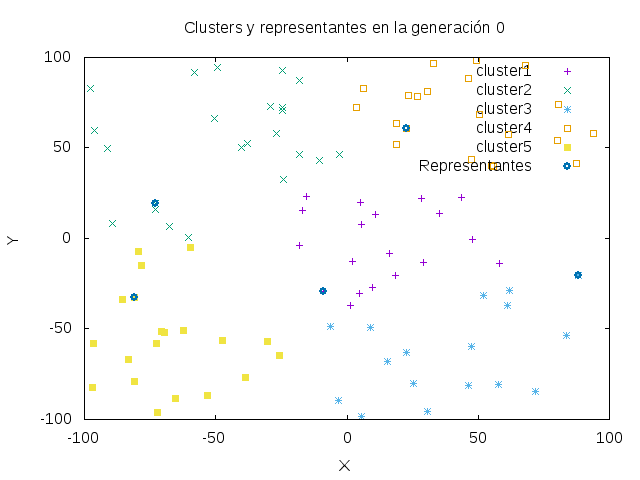
\includegraphics[width=0.7\linewidth]{graficos/0out}
\caption{Coste mínimo: 32.063385819971245}
\label{fig:0out}
\end{figure}

En esta primera generación de ideas aleatorias se tienen separados por colores cada uno de los clusters anteriormente dichos. Cada uno de ellos tiene un punto azul, el cuál es su representante de clase. Es la idea que, dentro de su cluster, tiene menor coste. Esos puntos será donde centraremos nuestra búsqueda y actuarán como punto de atracción.\\

\begin{figure}[H]
\centering
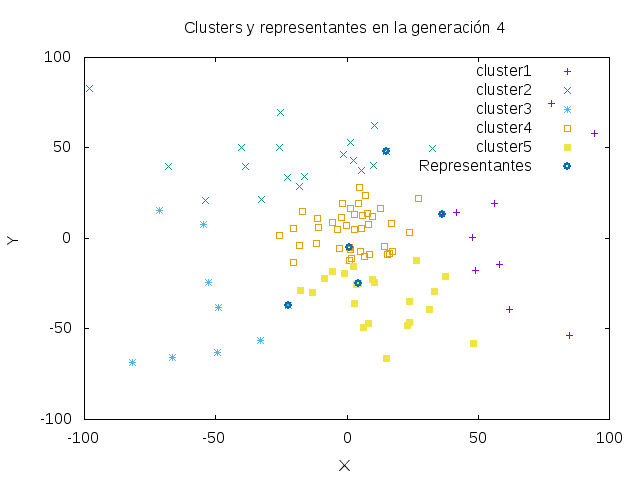
\includegraphics[width=0.7\linewidth]{graficos/4out}
\caption{Coste mínimo: 10.868608361185013}
\label{fig:1out}
\end{figure}

Tras unas cuantas generaciones vemos que se han agrupado ligeramente en el centro unos cuantos puntos (que es donde sabemos que la función de coste tiene un mínimo). Por último, en la última generación:\\

\begin{figure}[H]
\centering
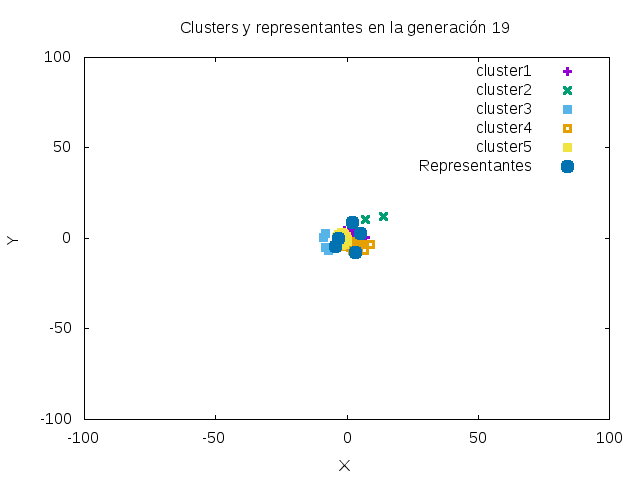
\includegraphics[width=0.7\linewidth]{graficos/19out}
\caption{Coste mínimo: 0.20025825415018517}
\label{fig:19out}
\end{figure}

se observa que se han agrupado todavía más en el centro. 


\section{Experimento y análisis de resultados.}

Para probar la bondad de este algoritmo vamos a compararlos con los resultados de la competición cec2014. Para empezar, aquí tenemos los resultados de nuestro algoritmo para las distintas dimensiones:\\

\textbf{Dimensión 10}

\begin{table}[htbp]
	\begin{center}
		\begin{tabular}{|l|l|}
			\hline
			Función & MejorCoste \\
			\hline \hline
			1 & 1183474.3628089789\\ \hline
			2 & 68864449.62907574 \\ \hline
			3 & 12052.281460498438 \\ \hline
			4 & 69.51174869048253 \\ \hline
			5 & 20.248590712702935 \\ \hline
			6 & 7.753179595914844 \\ \hline
			7 & 3.037059227484292 \\ \hline
			8 & 37.275446377989056 \\ \hline
			9 & 43.98963821630082 \\ \hline
			10 & 1000.5484210292489 \\ \hline
			11 & 1113.7294002188828 \\ \hline
			12 & 0.6969247915296819 \\ \hline
			13 & 0.307090955059266 \\ \hline
			14 & 0.48214180040963583 \\ \hline
			15 & 7.174151442472294 \\ \hline
			16 & 3.337923901207205 \\ \hline
			17 & 5020.6204587966295 \\ \hline
			18 & 1390.9914594921079 \\ \hline
			19 & 4.2737342582693145 \\ \hline
			20 & 418.4109712910604 \\ \hline
			
		\end{tabular}
		\caption{Datos obtenidos para el algoritmo BSO en dimensión 10}
		\label{tabla:Dimension10}
	\end{center}
\end{table}

\newpage
\textbf{Dimensión 30}
\begin{table}[htbp]
	\begin{center}
		\begin{tabular}{|l|l|}
			\hline
			Función & MejorCoste \\
			\hline \hline
			1 & 43298536.59965883 \\ \hline
			2 & 2231702882.802855 \\ \hline
			3 & 44340.855204072 \\ \hline
			4 & 484.2593344162864 \\ \hline
			5 & 21.014668359837742 \\ \hline
			6 & 36.26514427636721 \\ \hline
			7 & 22.793786929147018 \\ \hline
			8 & 225.40551388712902 \\ \hline
			9 & 244.94884716959336 \\ \hline
			10 & 6281.0562826495025 \\ \hline
			11 & 6509.02717523838 \\ \hline
			12 & 2.492430854865006 \\ \hline
			13 & 0.5413319342403611 \\ \hline
			14 & 5.876378892491402 \\ \hline
			15 & 86.47807547500452 \\ \hline
			16 & 12.791946204717078 \\ \hline
			17 & 395910.80626148934 \\ \hline
			18 & 2706236.20155882 \\ \hline
			19 & 27.90797550449406 \\ \hline
			20 & 16593.066630701265 \\ \hline

\end{tabular}
\caption{Datos obtenidos para el algoritmo BSO en dimensión 30}
\label{tabla:Dimension30}
\end{center}
\end{table}

\newpage

\textbf{Dimensión 50}

\begin{table}[htbp]
	\begin{center}
		\begin{tabular}{|l|l|}
			\hline
			Función & MejorCoste \\
			\hline \hline
			1& 34697256.464061595 \\ \hline
			2& 5435907284.533975 \\ \hline
			3& 144550.6975283996 \\ \hline
			4& 765.041913418198 \\ \hline
			5& 21.149918238175587 \\ \hline
			6& 66.01304943149626 \\ \hline
			7& 60.20723977810894 \\ \hline
			8& 488.14993516562254 \\ \hline
			9& 513.0639386330843 \\ \hline
			10& 12725.468378250636 \\ \hline
			11& 12293.26098058094 \\ \hline
			12 & 3.0114010897066237 \\ \hline
			13 & 0.5664698751006654 \\ \hline
			14 & 2.605832169932455 \\ \hline
			15 & 367.4337953141685 \\ \hline
			16 & 22.657877211097002 \\ \hline
			17 & 1510087.120038229 \\ \hline
			18 & 1511539.8969205872 \\ \hline
			19 & 53.3869744775036 \\ \hline
			20 & 45819.71571083536 \\ \hline
			
		\end{tabular}
		\caption{Datos obtenidos para el algoritmo BSO en dimensión 50}
		\label{tabla:Dimension50}
	\end{center}
\end{table}


\newpage

\subsection{Análisis de resultados}

Como no se nos ha dado ningún método general para comparar el algoritmo con el resto de Metaheurísticas, hemos escogido compararlas con el máximo y el mínimo de cada instancia, viendo así si está en el rango de la competición:\\

\begin{table}[htbp]
	\begin{center}
		\begin{tabular}{|l|l|l|}
			\hline
			Mínimo & Máximo & BSO \\
			\hline \hline
			0 & 8810740 & 731803,194310743 \\ \hline
			0 & 224053205,940771 & 74497204,3215033 \\ \hline
			0 & 6643,67 & 8897,2278282812 \\ \hline
			0 & 52,5332862745 & 66,3409061102 \\ \hline
			13,6519611765 & 20,2129862745 & 20,4042840546\\ \hline
			0 & 3,0166234 & 8,1117725686\\ \hline
			0 & 3,3068928078 & 1,9737411053\\ \hline
			0 & 18,904 & 29,1640036507\\ \hline
			2,344597678 & 21,0368678431 & 27,1556003416\\ \hline
			0,0085721782 & 330,8470785997 & 999,0282517068\\ \hline
			20,1349725373 & 782,9861372549 & 1496,061879948\\ \hline
			0 & 0,8030774706 & 0,9494295338\\ \hline
			0,0094357808 & 0,4161575699 & 0,4953625289\\ \hline
			0,081361704 & 0,6884131745 & 0,376404398\\ \hline
			0,3660991591 & 47,0112827255 & 5,8196928933\\ \hline
			1,054166198 & 2,8261445098 & 3,6320886826\\ \hline
			0,9766637611 & 3122910 & 2921,6764508118\\ \hline
			0,2440927767 & 225413,487599239 & 1327,892909848\\ \hline
			0,0766073275 & 2,3744214902 & 4,2782585716\\ \hline
			0,1848826079 & 9364,2 & 566,1684495604\\ \hline
			
			
		\end{tabular}
		\caption{Comparacin de BSO con las MH del cec2014. Dimensin 10}
		\label{tabla:Dimension10Comparativa}
	\end{center}
\end{table}

En esta primera tabla se observa que los valores máximos de coste de todas las metaheurísticas del cec son superadas en alguna de las funciones que evaluan. Sin embargo, comparar con el máximo de las demás funciones es injusto(Cada MH tiene sus puntos fuertes y puede que la peor MH de una instancia sea la mejor en otra). Por descontado, no se acerca al mínimo coste obtenido.\\

Esta tabla nos hace pensar que nuestra MH no es tan buena como podría parecer en un principio. Veamos las dos tablas siguientes.

\newpage


\begin{table}[htbp]
	\begin{center}
		\begin{tabular}{|l|l|l|}
			\hline
			Mínimo & Máximo & BSO \\
			\hline \hline
			0 & 215525900 & 43298536,5996588 \\ \hline
			0 & 517280687,246079 & 2231702882,80285\\ \hline
			0 & 10810,2 & 44340,855204072\\ \hline
			0 & 109,346 & 484,2593344163\\ \hline
			19,9995564118 & 20,6376972549 & 21,0146683598\\ \hline
			0 & 21,986927451 & 36,2651442764\\ \hline
			0 & 4,0912666823 & 22,7937869291\\ \hline
			0 & 92,531 & 225,4055138871\\ \hline
			6,7848764763 & 137,1473289608 & 244,9488471696\\ \hline
			0,0163288218 & 2312,38 & 6281,0562826495\\ \hline
			1229,4790938139 & 3877,6982352941 & 6509,0271752384\\ \hline
			0,0021532762 & 0,9895080784 & 2,4924308549\\ \hline
			0,0568129615 & 0,5608331353 & 0,5413319342\\ \hline
			0,1866163365 & 1,0154932941 & 5,8763788925\\ \hline
			2,1463695397 & 182,0982880392 & 86,478075475\\ \hline
			8,4990146629 & 11,4669638132 & 12,7919462047\\ \hline
			187,5081400917 & 28114700 & 395910,806261489\\ \hline
			5,9100668314 & 3170488,26827255 & 2706236,20155882\\ \hline
			3,0799649137 & 183,62 & 27,9079755045\\ \hline
			3,0818629205 & 38149,6 & 16593,0666307013\\ \hline
			
		\end{tabular}
		\caption{Comparación de BSO con las MH del cec2014. Dimensión 30}
		\label{tabla:Dimension30Comparativa}
	\end{center}
\end{table}

\begin{table}[htbp]
	\begin{center}
		\begin{tabular}{|l|l|l|}
			\hline
			Mínimo & Máximo & BSO \\
			\hline \hline
			0 & 53493400 & 34697256,4640616 \\ \hline
			0 & 680874996,911058 & 5435907284,53397 \\ \hline
			0 & 12152,1 & 144550,6975284 \\ \hline
			0 & 283,718 & 765,0419134182 \\ \hline
			19,9999054902 & 20,9904990196 & 21,1499182382 \\ \hline
			0,0882397243 & 41,8656921569 & 66,0130494315 \\ \hline
			0 & 7,7470206788 & 60,2072397781 \\ \hline
			6,70975258823529E-13 & 161,1830192307 & 488,1499351656 \\ \hline
			11,4467834745 & 247,0608935294 & 513,0639386331 \\ \hline
			0,121883502 & 4459,67 & 12725,4683782506 \\ \hline
			3221,9432146859 & 7969,801372549 & 12293,2609805809 \\ \hline
			0,0012733153 & 1,8487529216 & 3,0114010897 \\ \hline
			0,0970215283 & 0,604618111 & 0,5664698751 \\ \hline
			0,2375031416 & 1,1130047451 & 2,6058321699 \\ \hline
			4,7984972745 & 276,3205568627 & 367,4337953142 \\ \hline
			16,8540272323 & 20,6335653232 & 22,6578772111 \\ \hline
			664,7713339608 & 191613300 & 1510087,12003823 \\ \hline
			34,0114004902 & 1757141,30709804 & 1511539,89692059 \\ \hline
			6,7580719765 & 82,48 & 53,3869744775 \\ \hline
			13,9138033956 & 110331 & 45819,7157108354 \\ \hline
			
			
		\end{tabular}
		\caption{Comparación de BSO con las MH del cec2014. Dimensión 50}
		\label{tabla:Dimension50Comparativa}
	\end{center}
\end{table}

\newpage

Tras observar los resultados en dimensiones 30 y 50 nos damos cuenta que la superación de la función de coste del máximo de las MH por parte del BSO se convierte en algo anecdótico. En dimensión 10 se ha logrado competir con la peor MH del cec de cada instancia llegando a superarla varias veces. Sin embargo en dimensiones mayores, no se ha logrado el objetivo de batirla.
\newpage


\subsection{Posibles mejoras de los algoritmos}
A continuación se proponen distintas formas de llegar a mejorar la metaheuristica BSO.
\begin{itemize}
	\item La primera mejora que hemos aplicado en la práctica es el uso del cruce de Differential Evolution. En el paper no daban ninguna idea de cómo habían implementado ellos esta parte.
	
	\item El algoritmo de clustering se puede llegar a cambiar por otras técnicas.
	
	\item Se debería de poder crear más o menos ideas o clusters dependiendo del tamaño del problema. Hay que afinar cuanta $diversidad/intensidad$ aporta el número de ideas y clusters con respecto a la dimensión del problema.
	
	\item No hay ninguna razón por la que los parámetros escogidos para las probabilidades sean óptimos o si no debieran de variar con el tiempo. La probabilidad de intensificación podría aumentar cuando estemos cerca del máximo de evaluaciones, por ejemplo.
	
	\item En el algoritmo se dice que sólo se puede cambiar una idea por otra generada por ella y QUE LLEVE EL MISMO ÏNDICE, esto es, que si en el cruce la primera idea padre no es peor que el hijo no se reemplaza, dando igual los costes de los otros padres implicados. Quizás este comportamiento podría mejorarse haciendo que compitan por entrar en la nueva población de ideas.
	
	\item Puesto que la mutación sólo se hace efectiva si esta mejora a la idea actual, podríamos seguir aplicando esta mutación mientras nos dé mejores ideas y así intensificar la búsqueda.
\end{itemize}

Cabe destacar también por qué la aplicación de búsquedas locales no las considero:

\begin{itemize}
	\item En el propio algoritmo, con la mutación ofrecida y la característica de reemplazo directo del algoritmo, ya se está aplicando búsqueda local. Una idea no será reemplazada por una peor en ningún caso. 
	
	\item Tras una serie de pruebas hemos visto que el algoritmo genera rápido $N$ nuevas ideas al principio pero que conforme avanza, gasta alrededor del 50\% de las evaluaciones en la última generación(en las pruebas de dimensión 2). En esta etapa alrededor de la mitad de las veces probará a mutar soluciones. Puesto que no se han generado nuevos individuos en esta última etapa, es lógico pensar que las mutaciones no han tenido éxito, nos encontramos en un óptimo local. La búsqueda local intensificaría este comportamiento y quitaría diversidad al algoritmo.
\end{itemize}

\newpage
\begin{thebibliography}{9}
	\bibitem{BSO} 2011 - BSO (IJSIR) -Brain Storm Optimization Algorithm\\
	
	\bibitem{smith} Smith, R.: The 7 Levels of Change, 2nd edn. Tapeslry Press (2002)\\
	
\end{thebibliography}


\end{document}





